\documentclass[margin=5mm]{standalone}
\usepackage[dvipsnames]{xcolor}
\usepackage{pgfplots}
\usepackage{tikz}
\usepackage[tikz]{ocgx2}

\pgfplotsset{compat=1.18}
\begin{document}

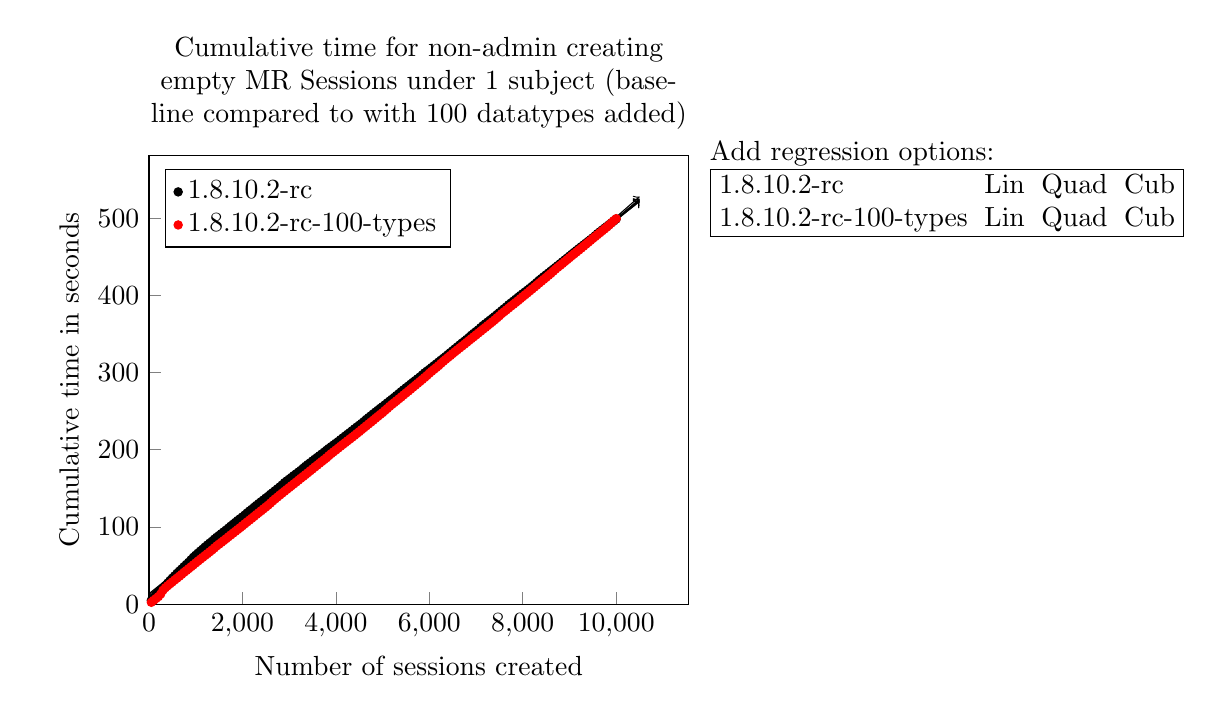
\begin{tikzpicture}
    \begin{axis}[
        align = center,
        legend pos = north west,
        legend cell align = left,
        xlabel = Number of sessions created,
        ylabel = Cumulative time in seconds,
        xtick pos = left,
        ytick pos = left,
        scaled ticks = false,
        xmin = 0,
        ymin = 0,
        title = {Cumulative time for non-admin creating empty MR Sessions under 1 subject  (baseline compared to with 100 datatypes added)},
        title style = {text width = 0.8\textwidth},
        legend entries={\switchocg{1.8.10.2-rc}{1.8.10.2-rc},\switchocg{1.8.10.2-rc-100-types}{1.8.10.2-rc-100-types}}]
        \begin{scope}[ocg = {ref = 1.8.10.2-rc-Lin, status = invisible}]
            \plot[domain=0:10500,->,forget plot] (\x,{13.5022689949745515747281388030387461185455322265625 + 0.04858249771244287085192326003380003385245800018310546875*(\x)^1});
        \end{scope}
        \begin{scope}[ocg = {ref = 1.8.10.2-rc-Quad, status = invisible}]
            \plot[domain=0:10500,->,forget plot] (\x,{11.7977840398961024703794464585371315479278564453125 + 0.0495950630322914698400182942350511439144611358642578125*(\x)^1 + -0.00000010075276814413957790259154974343847044337962870486080646514892578125*(\x)^2});
        \end{scope}
        \begin{scope}[ocg = {ref = 1.8.10.2-rc-Cub, status = invisible}]
            \plot[domain=0:10500,->,forget plot] (\x,{7.74289272441223630494278040714561939239501953125 + 0.054377196327513845075518617022680700756609439849853515625*(\x)^1 + -0.00000128737657407024623298506978141819701022541266866028308868408203125*(\x)^2 + 0.00000000007871468032677323468471219621291567157539414978373315534554421901702880859375*(\x)^3});
        \end{scope}
        \begin{scope}[ocg = {ref = 1.8.10.2-rc, status = visible}]
            \addplot[
                only marks,
                color = black,
                mark = *,
                mark size = 1.5 pt
            ]coordinates {(50,4.877)(100,8.334)(150,11.626)(200,14.859)(250,17.838)(300,20.884)(350,23.96)(400,27.212)(450,30.602)(500,33.768)(550,36.695)(600,39.884)(650,42.829)(700,45.599)(750,48.598)(800,51.416)(850,54.215)(900,57.468)(950,60.695)(1000,63.358)(1050,66.091)(1100,68.762)(1150,71.219)(1200,74)(1250,76.622)(1300,79.062)(1350,81.415)(1400,84.198)(1450,86.66)(1500,88.975)(1550,91.286)(1600,93.643)(1650,95.982)(1700,98.438)(1750,101.023)(1800,103.483)(1850,105.878)(1900,108.387)(1950,110.677)(2000,112.99)(2050,115.445)(2100,118.068)(2150,120.609)(2200,122.87)(2250,125.466)(2300,127.893)(2350,130.339)(2400,132.658)(2450,134.966)(2500,137.372)(2550,139.633)(2600,142.235)(2650,144.474)(2700,146.974)(2750,149.413)(2800,151.855)(2850,154.392)(2900,157.334)(2950,159.595)(3000,161.882)(3050,164.15)(3100,166.53)(3150,168.748)(3200,171.105)(3250,173.318)(3300,175.974)(3350,178.503)(3400,180.841)(3450,183.046)(3500,185.482)(3550,187.739)(3600,190.046)(3650,192.224)(3700,194.532)(3750,196.89)(3800,199.336)(3850,201.668)(3900,203.892)(3950,206.11)(4000,208.347)(4050,210.609)(4100,213.004)(4150,215.328)(4200,217.694)(4250,220.016)(4300,222.296)(4350,224.709)(4400,227.075)(4450,229.435)(4500,231.719)(4550,234.042)(4600,236.561)(4650,239.239)(4700,241.574)(4750,244.014)(4800,246.428)(4850,248.811)(4900,251.177)(4950,253.594)(5000,255.81)(5050,258.216)(5100,260.609)(5150,262.956)(5200,265.371)(5250,267.755)(5300,270.258)(5350,272.736)(5400,275.29)(5450,277.632)(5500,280.118)(5550,282.483)(5600,284.877)(5650,287.275)(5700,289.596)(5750,291.9)(5800,294.258)(5850,296.944)(5900,299.529)(5950,301.865)(6000,304.078)(6050,306.455)(6100,308.892)(6150,311.225)(6200,313.614)(6250,316.038)(6300,318.432)(6350,320.799)(6400,323.388)(6450,325.822)(6500,328.277)(6550,330.811)(6600,333.26)(6650,335.728)(6700,338.217)(6750,340.556)(6800,342.976)(6850,345.498)(6900,348.309)(6950,350.662)(7000,353.059)(7050,355.414)(7100,358.113)(7150,360.817)(7200,363.134)(7250,365.448)(7300,367.867)(7350,370.219)(7400,372.603)(7450,375.183)(7500,377.556)(7550,380.114)(7600,382.65)(7650,385.099)(7700,387.796)(7750,390.129)(7800,392.498)(7850,394.926)(7900,397.422)(7950,399.782)(8000,402.049)(8050,404.397)(8100,406.705)(8150,409.066)(8200,411.568)(8250,413.998)(8300,416.595)(8350,419.384)(8400,421.736)(8450,424.174)(8500,426.568)(8550,428.894)(8600,431.322)(8650,433.732)(8700,436.136)(8750,438.491)(8800,440.952)(8850,443.387)(8900,445.851)(8950,448.268)(9000,450.732)(9050,453.228)(9100,455.7)(9150,458.086)(9200,460.458)(9250,462.783)(9300,465.123)(9350,467.475)(9400,469.886)(9450,472.234)(9500,474.585)(9550,477.189)(9600,479.922)(9650,482.238)(9700,484.613)(9750,486.934)(9800,489.244)(9850,491.625)(9900,494.08)(9950,496.454)(10000,498.871)};
        \end{scope}
        \begin{scope}[ocg = {ref = 1.8.10.2-rc-100-types-Lin, status = invisible}]
            \plot[domain=0:10500,->,forget plot] (\x,{2.256911407035143923849318525753915309906005859375 + 0.049514953948848729192722117886660271324217319488525390625*(\x)^1});
        \end{scope}
        \begin{scope}[ocg = {ref = 1.8.10.2-rc-100-types-Quad, status = invisible}]
            \plot[domain=0:10500,->,forget plot] (\x,{3.6735846710826702832264345488511025905609130859375 + 0.048673365871196742904469800805600243620574474334716796875*(\x)^1 + 0.0000000837401072290525966539893377472980606768260258832015097141265869140625*(\x)^2});
        \end{scope}
        \begin{scope}[ocg = {ref = 1.8.10.2-rc-100-types-Cub, status = invisible}]
            \plot[domain=0:10500,->,forget plot] (\x,{3.254401328145043681416836989228613674640655517578125 + 0.049167729459540010505946838748059235513210296630859375*(\x)^1 + -0.00000003892974877375738191564484504299248346370632134494371712207794189453125*(\x)^2 + 0.00000000000813730388078341327609674247506158818732391324601849191822111606597900390625*(\x)^3});
        \end{scope}
        \begin{scope}[ocg = {ref = 1.8.10.2-rc-100-types, status = visible}]
            \addplot[
                only marks,
                color = red,
                mark = *,
                mark size = 1.5 pt
            ]coordinates {(50,2.396)(100,4.855)(150,7.264)(200,9.66)(250,13.063)(300,18.084)(350,21.219)(400,23.803)(450,26.34)(500,28.786)(550,31.261)(600,33.682)(650,36.136)(700,38.575)(750,41.186)(800,43.554)(850,45.952)(900,48.414)(950,50.83)(1000,53.312)(1050,55.842)(1100,58.246)(1150,60.612)(1200,63.022)(1250,65.34)(1300,67.745)(1350,70.181)(1400,72.803)(1450,75.424)(1500,77.756)(1550,80.063)(1600,82.361)(1650,84.701)(1700,87.223)(1750,89.556)(1800,91.978)(1850,94.332)(1900,96.691)(1950,99.038)(2000,101.507)(2050,103.945)(2100,106.412)(2150,108.803)(2200,111.21)(2250,113.625)(2300,116.173)(2350,118.493)(2400,120.896)(2450,123.366)(2500,125.738)(2550,128.18)(2600,130.893)(2650,133.674)(2700,136.289)(2750,138.74)(2800,141.269)(2850,143.744)(2900,146.151)(2950,148.563)(3000,150.987)(3050,153.367)(3100,155.739)(3150,158.121)(3200,160.592)(3250,163.045)(3300,165.373)(3350,167.763)(3400,170.175)(3450,172.68)(3500,175.049)(3550,177.62)(3600,179.974)(3650,182.424)(3700,184.812)(3750,187.197)(3800,189.555)(3850,192.352)(3900,194.916)(3950,197.246)(4000,199.631)(4050,202.044)(4100,204.448)(4150,206.823)(4200,209.226)(4250,211.557)(4300,213.871)(4350,216.219)(4400,218.587)(4450,221.054)(4500,223.428)(4550,225.972)(4600,228.397)(4650,230.875)(4700,233.311)(4750,235.751)(4800,238.206)(4850,240.761)(4900,243.212)(4950,245.691)(5000,248.073)(5050,250.833)(5100,253.356)(5150,256.129)(5200,258.661)(5250,261.053)(5300,263.44)(5350,265.908)(5400,268.38)(5450,270.923)(5500,273.451)(5550,275.886)(5600,278.398)(5650,280.938)(5700,283.407)(5750,285.96)(5800,288.437)(5850,290.997)(5900,293.564)(5950,296.135)(6000,299.02)(6050,301.596)(6100,304.032)(6150,306.47)(6200,308.968)(6250,311.851)(6300,314.543)(6350,317.055)(6400,319.556)(6450,321.964)(6500,324.493)(6550,327)(6600,329.418)(6650,331.804)(6700,334.2)(6750,336.599)(6800,339.012)(6850,341.472)(6900,343.848)(6950,346.255)(7000,348.686)(7050,351.17)(7100,353.568)(7150,356.008)(7200,358.405)(7250,360.842)(7300,363.319)(7350,365.771)(7400,368.18)(7450,370.86)(7500,373.478)(7550,376.327)(7600,378.706)(7650,381.124)(7700,383.584)(7750,386.1)(7800,388.368)(7850,390.742)(7900,393.165)(7950,395.736)(8000,398.213)(8050,400.691)(8100,403.144)(8150,405.659)(8200,408.178)(8250,410.683)(8300,413.185)(8350,415.811)(8400,418.276)(8450,420.75)(8500,423.229)(8550,425.813)(8600,428.287)(8650,431.125)(8700,433.766)(8750,436.301)(8800,438.76)(8850,441.193)(8900,443.74)(8950,446.224)(9000,448.718)(9050,451.261)(9100,453.692)(9150,456.084)(9200,458.548)(9250,461.024)(9300,463.476)(9350,466.039)(9400,468.552)(9450,471.088)(9500,473.648)(9550,476.098)(9600,478.564)(9650,481.012)(9700,483.525)(9750,485.916)(9800,488.444)(9850,491.079)(9900,493.914)(9950,496.712)(10000,499.257)};
        \end{scope}
    \end{axis}
    \begin{scope}
        \addtolength{\tabcolsep}{-0.3em}
        \node [below right, shape=rectangle, align=left](regressiontable) at (7,6) {
            Add regression options: \\
            \begin{tabular}{|llll|}
                \hline
                1.8.10.2-rc & \switchocg{1.8.10.2-rc-Lin}{Lin} & \switchocg{1.8.10.2-rc-Quad}{Quad} & \switchocg{1.8.10.2-rc-Cub}{Cub} \\
                1.8.10.2-rc-100-types & \switchocg{1.8.10.2-rc-100-types-Lin}{Lin} & \switchocg{1.8.10.2-rc-100-types-Quad}{Quad} & \switchocg{1.8.10.2-rc-100-types-Cub}{Cub} \\
                \hline
            \end{tabular}
        };
    \end{scope}
\end{tikzpicture}

\end{document}